\section{Linked Data}
\label{sec:linked_data}

Het semantisch web gaat echter niet enkel over het plaatsen van data op het web. Het belangrijkste aspect van het semantisch web is het maken van links, zodat zowel personen als machines het web van data kunnen doorkruisen. Het belangrijke aan gelinkte data kan als volgt omschreven worden: wanneer je data hebt, kan je er elders andere gerelateerde data mee vinden. Op deze manier wordt context aan de data meegegeven. Bij gelinkte data worden deze links beschreven aan de hand van RDF. Hierbij worden URI's gebruikt voor het identificeren van objecten. Om data te interconnecteren zijn er vier regels, met als doel dat de informatie in de toekomst op onvoorspelbare manieren herbruikt zou kunnen worden. Daarnaast is het belangrijk dat de data open en toegankelijk zijn om herbruikt te worden \cite{berners2006linkeddata}. 

\subsection{Regels}
Bij gelinkte data zijn er vier regels waaraan voldaan moet worden:
\begin{enumerate}
    \item Objecten moeten geïdentifeceerd worden met URI's. Dit is nodig om te kunnen spreken over een semantisch web \cite{berners2006linkeddata}. 
    \item Er moet gebruik gemaakt worden van \acrfull{http} URI's. Dit is nodig zodat andere gebruikers de namen zouden kunnen opzoeken \cite{berners2006linkeddata}. 
    \item Bijhorende informatie moet gevonden kunnen worden wanneer een URI gevolgd wordt. Dit is in het basisformaat van RDF en XML. Deze kan ook doorzocht worden aan de hand van SPARQL (verder besproken in \sectionref{sec:sparql}), dit is een query service voor gelinkte data in RDF formaat \cite{berners2006linkeddata}. 
    \item Er moeten links voorzien worden naar andere locaties die gelijkaardige data bevatten, zodat deze opgezocht kunnen worden. Deze laatste regel is belangrijk om de informatie op het web te connecteren \cite{berners2006linkeddata}.
\end{enumerate}

\subsection{Vijfsterrenmodel}
Het vijfsterrenmodel is een manier om informatie in te delen op basis van openheid. Meer sterren betekent dat de informatie meer open is. Tim Berners-Lee stelde dit model voor als schema voor gelinkte open data. Gelinkte open data is een essentiëel onderdeel van het semantisch web.

Eén ster stelt hetvolgende: ``\textit{Available on the web but with an open licence, to be Open Data}''. Dit betekent dat gebruikers informatie kunnen ophalen, gebruiken en delen met iedereen. Het gaat hier echter louter over het delen van informatie, het maakt dus niet uit in welk formaat dit komt \cite{berners2006linkeddata}. 

Twee sterren stelt dan weer: ``\textit{Available as machine-readable structured data}''. Om twee sterren te krijgen is het belangrijk dat de informatie een bepaalde structuur heeft, zodat machines deze informatie kunnen verwerken. Dit kan bijvoorbeeld zijn in de vorm van een excel spreadsheet. Dit soort informatie is echter nog steeds vrij gesloten aangezien de gebruikers afhankelijk zijn van bepaalde software om toegang te krijgen tot de informatie \cite{berners2006linkeddata}.

Drie sterren betekent: ``\textit{The same as 2 stars, plus non-proprietary format}''. Het verschil om van twee sterren naar drie sterren te stijgen is het vermijden van de nood aan specifieke software om de informatie te bemachtigen. Dit kan bijvoorbeeld door de informatie op te slaan in \acrfull{csv} formaat \cite{berners2006linkeddata}.

Vier sterren is vervolgens: ``\textit{All the above plus, use open standards from \acrshort{w3c} to identify things, so that people can point at your stuff}''. Om een vierde ster te verdienen moet de informatie voldoen aan de open standaarden van \acrshort{w3c}. Zo moet het objecten identificeren aan de hand van RDF of SPARQL. Hierbij is het belangrijk dat gebruikers (aan de hand van URI) kunnen verwijzen naar de data \cite{berners2006linkeddata}.

Tenslotte betekent vijf sterren het volgende: ``\textit{All the above, plus: Link your data to other people’s data to provide context}''. Om de laatste ster ook te kunnen behalen, dient men de informatie te linken aan bijhorende informatie in een andere context. Op deze manier worden de links verder verspreid. Hier wordt er dus letterlijk verwezen naar andere locaties, met als doel om meer context terug te vinden \cite{berners2006linkeddata}.

\subsection{Linked data gevisualiseerd}

\begin{figure}[ht!]
    \centering
    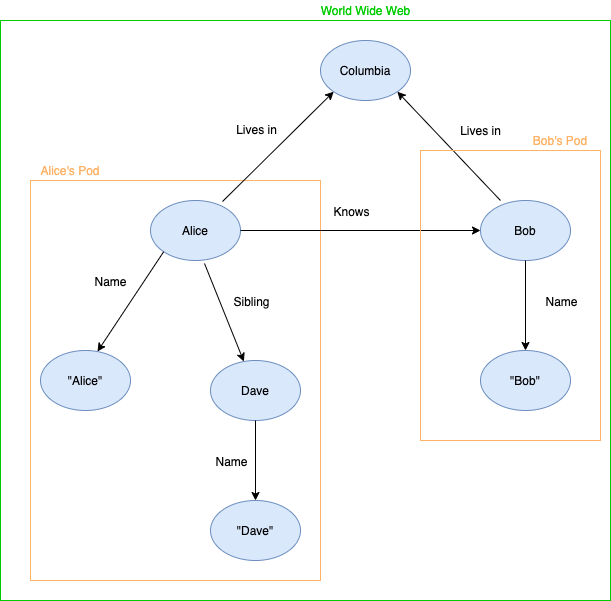
\includegraphics[width=\linewidth]{Linked-Data-Example.png}
    \caption{Voorbeeld van Linked Data.}
    \label{fig:linked_data_example}
\end{figure}

Een voorbeeld van hoe het \textit{World Wide Web} eruit zou kunnen zien is geschetst in \figureref{fig:linked_data_example}. Dit voorbeeld toont de ideale situatie waar personen een eigen pod met informatie hebben. Zo hebben Alice en Bob elk hun eigen plaats in het web, waar informatie over hun te vinden is. Deze informatie zou onder andere hun naam, telefoonnummer, adres, interesses, werkomgeving, etc kunnen zijn. Daarnaast zijn er ook connecties tussen Alice en Bob. Om te beginnen is Bob gekend door Alice, waardoor er een verwijzing is naar meer context over Bob in zijn pod. Daarnaast wonen ze beide in dezelfde stad, waardoor het mogelijk is om bijvoorbeeld te zoeken naar iedereen die in een bepaalde stad woont. Al deze personen zullen terug te vinden zijn aan de hand van een verwijzing naar meer context (lees: meer informatie) gelinkt aan personen. Dit is echter een vereenvoudigd voorbeeld, in de reële situatie zijn er veel meer links en dit in meerdere richtingen.